\chapter*{Background}

This chapter provides the background on the broader context of the problem addressed by this thesis. It covers a brief history of the standardization efforts as well as a review of the literature in the research domain relevant to this thesis, including \acp{PON}, network sharing, virtualization, and blockchain technology. In section \ref{Back:Sec:PON}, we briefly introduce \acp{PON} that form the main scope of this thesis. In subsection \ref{Back:Sec:PON:sub:DBA} we provide a brief review of the \ac{DBA} algorithms. Section \ref{Back:Sec:sharing} introduces the main theme of this thesis that is network sharing and investigates the technological and economic challenges associated with it. In Section \ref{Back:Sec:Virtualazation}, we review network virtualization and \ac{SDN} as technological enablers of network sharing. Section \ref{Back:Sec:auction} lays out the theoretical dimension of game-theoretical approaches towards resource sharing problems in telecommunications with a focus on auction mechanisms. Finally, in section \ref{Back:Sec:blockchain} provides an introduction to blockchain technology accompanied by a brief overview of its solution to the trust-less business ecosystems.


%%%%%%%%%%%%%%%%%%%%%%%%%%%%%%%%%%%%%%%%%%%%%%%%%%%%%%%%%%
%%%%%%%%%%%%%%%%%%%%%%%%%%%%%%%%%%%%%%%%%%%%%%%%%%%%%%%%%%
%%%%%%%%%%%%%%%%%%%%%%%%%SECTION%%%%%%%%%%%%%%%%%%%%%%%%%%
%%%%%%%%%%%%%%%%%%%%%%%%%%%%%%%%%%%%%%%%%%%%%%%%%%%%%%%%%%
%%%%%%%%%%%%%%%%%%%%%%%%%%%%%%%%%%%%%%%%%%%%%%%%%%%%%%%%%%
\section{\acf{PON}}
\label{Back:Sec:PON}
% \section{Access Networks}

Access networks are the most expensive part of telecommunication networks due to the massive number of network elements they require. Consequently, intensive research has been done, and many ingenious solutions have been provided for this vital part of the telecommunication networks. For over a decade, \ac{DSL} over copper dominated the fixed access market by providing point-to-point wired access to support each subscriber with up to 24 Mbit/s downstream using its most popular version ADSL2+ \cite{ituG.992.5}. Furthermore, in \ac{G.Fast}, they are targeting 500-1000 Mbit/s for local loops under 100 meters, and 150 Mbit/s for straight loops (local loop) without bridge taps up to a 250m distance from the subscriber \cite{ituG.9700}. Even though \ac{G.Fast} promises sufficient bandwidths, the substantial investment required for the active network equipment, and considering the short reach and a small number of subscribers the technology can support is unavoidable. Such solutions may be cost-effectively feasible for highly dense populated municipal areas but not for sparsely populated non-metropolitan regions.

On the one hand, these access technologies entail a considerable number of active network elements such as routers, switches, etc. and on the other hand, they are unable to fulfill subscribers' growing thirst for the bandwidth. Whereas, optical networks were getting more and more popular in core networks thanks to the vast bandwidth capability they were providing compared to their counterparts.

\acp{PON} are a series of fixed access network technologies that offer numerous advantages when deployed in \ac{FTTx} scenarios. The advantages include a point to multi-point architecture, high-quality triple play service capabilities for data, voice and video, high-speed Internet access, and other services in a cost-effective manner \cite{Abbas201653}.


\ac{PON}'s bandwidth management technique in downstream is similar to a simple broadcast network which broadcasts all the data to every \ac{ONU}, and then the relevant \ac{ONU} would be able to access its requested data. On the other hand, in the upstream direction in the worst case, all the \acp{ONU} want to send data over the single shared fiber with fixed bandwidth. The dynamic bandwidth allocation is responsible for making sure that no collision will occur, and the upstream bandwidth will be fairly shared among the \acp{ONU}. Furthermore, the bandwidth allocation process should respect the \ac{SLA}) and \ac{QoS}.

The point to multi-point nature of \ac{PON} enables the support of numerous users up to 1024 \acp{ONU}, and 125 Kilometers reach recently demonstrated \cite{7494070}. The available capacity reaches up to 10 Gbps symmetric rates per channel, with up to 8 channels in NG-PON2, with standardization efforts aiming at 25 Gbps per channel and research results showing rates of 100 Gbps. These characteristics of \ac{PON} make it a suitable candidate for being used as shared infrastructure. The flexible nature of \ac{PON} makes it an excellent infrastructure option for different environments from remote rural areas as one \ac{PON} can potentially support the entire traffic of a village to the dense traffic in the city center of a big city. However, sharing the \ac{PON} among multiple operators with potential service diversity demands a reliable quality of service scheme to guarantee sustainable service delivery to the end-users. i.e., the sharing shall not prevent the operators from implementing their \ac{QoS} scheme to satisfy diverse service-dependent requirements. Failing to provide this service differentiation in a \ac{PON} can break the chain of end-to-end \ac{QoS} and interfere with the traffic engineering capability of the operators.

The two standardization bodies, namely, \ac{IEEE} and \ac{ITU}, are in parallel developing standards for \acp{PON}. The two standards are known as \ac{EPON} and \ac{GPON}.


% Passive Optical Networks (PONs) are a series of promising broadband access network technologies that offer numerous advantages when deployed in fiber to the home (FTTH) scenarios. Those advantages include a point to multi-point architecture, high-quality triple play service capability for data, voice and video, high-speed Internet access, and other services in a cost-effective manner \cite{Abbas201653}.



The idea of \ac{EPON} was born by the formation of the \ac{IEEE} 802.3 study group called \ac{EFM} in November 2000 \cite{879000}. The group was to extend Ethernet into the subscriber access area. \ac{P2MP} fiber (also known as \ac{EPON}) was one of the focus areas of this group. The efforts of this group was reflected in \ac{IEEE} 802.3ah-2004 \cite{1337489} which were later included in the overall standard \ac{IEEE} 802.3-2008 \cite{4726971}, 2012 \cite{6419735} and the most recent amendment to it \ac{IEEE} 802.3bm-2015 \cite{7069180}.
\ac{EPON} technology provides bidirectional 1 Gb/s links using 1490 nm wavelength for downstream and 1310 nm for upstream, with 1550 nm reserved for future extensions or additional services, such as analog video broadcast \cite{4150568}.

Gigabit-capable \ac{PON} is a \ac{QoS}-enabled variant of \acp{PON} that has been standardized by the \ac{ITU} in the G-series recommendations. \ac{GPON} employs an embedded \ac{QoS} technique by defining logical queues called traffic containers for different service types with higher service frequency for delay-sensitive application and more significant transmission opportunities for bandwidth-hungry applications. \ac{GPON} is defined as ITU-T G.984 \cite{itu984} series of recommendations. More recent versions of this standard are known as \ac{XG-PON}, and \ac{NG-PON2} justified in ITU-T G.987 \cite{itu987} and ITU-T G.989 \cite{itu989} respectively.

\ac{XG-PON} and \ac{NG-PON2} are based on \ac{GPON} and inherit most of their features, including framing and management techniques from that with improvements in bit-rate and coverage. A \ac{GPON} system can typically accommodate 64 users at a maximum distance of 20km (OLT to ONT) with downstream/upstream rate of 2.5/1.25 Gbit/s while \ac{XG-PON} operate at 10/2.5 Gbit/s bandwidth and can increase the support to 128 users or increase the distance at 60km but not simultaneously. \ac{NG-PON2} takes the bandwidth to up to 40 Gbit/s symmetrically for both downstream and upstream thanks to the TWDM technique.

\subsection{\acf{DBA}}
\label{Back:Sec:PON:sub:DBA}

% \torephrase{\ac{PON}'s bandwidth management technique in downstream is similar to a simple broadcast network which broadcasts all the data to every \ac{ONU}, and then the related \ac{ONU} would be able to access its requested data. However, in the upstream direction, when in the worst case when all the \ac{ONU}'s want to send data over the single shared fiber with fixed bandwidth, the problem of how to allocate the bandwidth to each \ac{ONU} arises.
% }

% A noble bandwidth allocation technique should meet the following characteristics:


% \begin{enumerate}
% \item It should prevent any collision of the data from different \acp{ONU} as they share the \ac{ODN}'s upstream channel.
% \item The allocation should be fair to the \acp{ONU} so none of them should face bandwidth starvation.
% \item It has to meet \ac{QoS} requirements for prioritized applications and user classes defined by the network operator.
% \item The algorithm should be flexible so it can adapt to the instantaneous traffic demands of the \acp{ONU}.
% \item It Should Utilize the bandwidth efficiently.
% \item It Should minimize the delay.
% \end{enumerate}

% To satisfy these requirements, the algorithms should unquestionably be dynamic.
% The \ac{DBA} mechanisms have not had a radical change throughout the process of going from \ac{GPON} to \ac{NG-PON2} except for considering the dynamic wavelength assignment in \ac{NG-PON2}. However, the question of developing a coupled/decoupled Dynamic wavelength and bandwidth allocation (DWBA) is a question being addressed in research papers \cite{6647627,6958533,han2013performance,6647859} as it was left to the implementers' discretion in the ITU-T G.989 recommendation.

The best known \ac{DBA} algorithms for \ac{EPON} and \ac{GPON} are IPACT \cite{983911} and GIANT \cite{DAC:DAC761}, respectively. Skubic et.al have comprehensively compared the \ac{DBA} mechanisms of \ac{EPON} and \ac{GPON} in \cite{Skubic:2009:CDB:1669975.1669987}. \ac{ITU} considered the addition of the \ac{DBA} to its B-PON standards in recommendation G.983.4 \cite{ITU_g.983.4_nodate}. This recommendation specifies the requirements to equip broadband optical access systems defined in ITU-T Rec. G.983.1 \cite{ITU_g.983.1_nodate} with \ac{DBA} functionality where the concept of \ac{T-CONT} is defined, and the types are discussed in detail.

ITU-T G.989.3 \cite{ITU_g.989.3_nodate}, 40-Gigabit-capable passive optical networks (\ac{NG-PON2}): Transmission Convergence Layer Specification introduces the guidelines and principals for the upstream and downstream resource allocation along with the quality of service capabilities of the \ac{NG-PON2}. This recommendation presents a more mature and detailed description of the \ac{DBA} in general and concise mathematics to formulate the different types of bandwidth specified in the algorithm, such as guaranteed, non-assured, and best-effort. Furthermore, an extended bandwidth assignment model is introduced and demonstrated via a realizable architecture. The reference model imposes a strict priority hierarchy for different forms of assigned bandwidth. This hierarchy is the main building block of the \ac{NG-PON2}'s \ac{QoS} and contains the following traffic classes:

\begin{enumerate}
\item Fixed bandwidth (highest priority).
\item Assured bandwidth.
\item Non-assured bandwidth.
\item Best-effort bandwidth (lowest priority).
\end{enumerate}

Guaranteed bandwidth consists of fixed and assured bandwidth. The fixed bandwidth will be assigned first regardless of the \acp{ONU}' offered load and overall traffic; as a result, any excess bandwidth is wasted. Next, the assured bandwidth will be assigned up to the provisioned limit or the subject \ac{ONU}'s satisfaction. After allocating the guaranteed part of the bandwidth, the non-assured should be assigned until the exhaustion of the surplus bandwidth pool or saturation of the \ac{ONU}. The best-effort bandwidth then will be allocated to the \ac{ONU} if it is not saturated.

% The recommendation recommends three performance criteria to evaluate a \ac{DBA} algorithm:
% \begin{itemize}
% \item[--] Stationary bandwidth assignment: In a stationary state of the system with constant traffic demand from \ac{ONU}s, the assigned bandwidth should approach the average of the k (k should be large enough to represent the frame diversity) assignments in consecutive downstream frames.
% \\Target: The stationary assigned bandwidth should be bigger than or equal to the fixed plus assured bandwidth.
% \item[--] Assured bandwidth restoration time: The time that and \ac{ONU} has to wait before getting its full provisioned assured plus fixed bandwidth share once it demands it.
% \\Target: Two milliseconds.
% \item[--] \ac{DBA} convergence time: The time that takes the \ac{OLT} to assign fixed plus assured bandwidth once the system steps out of the stationary state.
% \\Target: six milliseconds.
% \end{itemize}


It is noteworthy that ITU-T G.989.3 \cite{ITU_g.989.3_nodate} inherits these specifications from the legacy \ac{ITU} standards ITU-T Rec. G.984.3 \cite{itu984} and ITU-T Rec. G.987.3 \cite{itu987} and most of the details about \ac{DBA} remains unchanged. Rather than mandating any specific \ac{DBA} algorithm, \ac{ITU} standards only specify control messages exchanges between \ac{ONU}s and the OLT. In particular, the \ac{DBA} process is not specified in detail by the manufacturers\cite{7333289}.



GigaPON Access Network (GIANT) \ac{MAC} method \cite{DAC:DAC761,Angelopoulos2004,1267106} an \ac{ITU} G.984.3 \cite{itu984} standard complaint \ac{DBA} algorithm is the baseline \ac{DBA} for most of the research papers on \ac{GPON} \ac{DBA}. GIANT implements the \ac{QoS} specifications of the standard using four different \acp{T-CONT} (traffic container) types. Each \acp{T-CONT} is served every service interval (SI) with certain allocation bytes (AB) based on their Queue occupancy reports.

% \begin{table}[tbp]
% \centering
% \caption{\ac{GPON} Traffic Types}
% \label{tbl:gpontraffic}
% \resizebox{1.0\textwidth}{!}{
% \begin{tabular}{|c|c|c|c|c|c|c|}
% \hline
% \textbf{TC}                 & \textbf{Applications}                                                               & \textbf{Throughput}                                                                & \textbf{Delay}   & \textbf{GPON service}                                                                & \textbf{MAC parameters}                                                    & \textbf{Traffic descriptors} \\ \hline
% \textbf{1}                  & \begin{tabular}[c]{@{}c@{}}Constant bit rate \\ (leased line)\end{tabular}          & Fixed                                                                              & Strict guarantee & Periodic upon activation                                                             & SImax, ABmin                                                               & PIR, PBS, Dm                 \\ \hline
% \textbf{2}                  & \begin{tabular}[c]{@{}c@{}}Variable bit rate\\  (voice, video)\end{tabular}         & Assured                                                                            & Bounded          & Periodic, validated by requests                                                      & SImax, ABmin                                                               & PIR, PBS, Dm                 \\ \hline
% \multirow{2}{*}{\textbf{3}} & \multirow{2}{*}{\begin{tabular}[c]{@{}c@{}}Better than \\ Best-Effort\end{tabular}} & Assured                                                                            & No guarantee     & Periodic, validated by requests                                                      & SImax, ABmin                                                               & GIR, GBS                     \\ \cline{3-7}
%                             &                                                                                     & \begin{tabular}[c]{@{}c@{}}Surplus allocated \\ dynamically up to PIR\end{tabular} &                  & \begin{tabular}[c]{@{}c@{}}Dynamic based on request\\  and availability\end{tabular} & SImin, ABsur                                                               & PIR, PBS                     \\ \hline
% \multirow{2}{*}{\textbf{4}} & \multirow{2}{*}{Best Effort}                                                        & No guarantee                                                                       &                  &                                                                                      & \begin{tabular}[c]{@{}c@{}}SImax, ABmin \\ (used for polling)\end{tabular} &                              \\ \cline{3-7}
%                             &                                                                                     & \begin{tabular}[c]{@{}c@{}}Dynamic assignment\\  up to PIR\end{tabular}            & No guarantee     & \begin{tabular}[c]{@{}c@{}}Dynamic based on request\\ and availability\end{tabular}  & SImin, ABsur                                                               & PIR, PBS                     \\ \hline
% \end{tabular}
% } %resizebox
% \end{table}


% In \cite{Han:08}, the authors have identified two drawbacks in GIANT, the first problem is associated with the service interval timer. In case a \ac{T-CONT} has a full buffer, but its SI counter has not expired, it will have to wait until the timer's expiration even if none of the other \acp{T-CONT} is not using the bandwidth. The immediate allocation technique proposed to overcome this problem. IA introduces a byte counter for each \ac{T-CONT} representing the remaining available allocation bytes. Using the byte counter, the algorithm will ignore the SI timer and will allocate bandwidth to the \ac{T-CONT} until its byte counter is zero while limiting the maximum allocation amount for a \ac{T-CONT} to lower than the value of the available byte counter.

% The second drawback is that because the scheduling decision in \ac{OLT} is based on the buffer occupancy report of the \ac{T-CONT} from the previous service interval, the current queue status of the \ac{T-CONT} can be different. So, in case one of the \acp{T-CONT} has new arrivals in its queue, it will not be assigned bandwidth since GIANT will assign bandwidth up to the requested amount. Colorless Grant (CG) has been introduced in \cite{Han:08} to utilize the unallocated remainder of the upstream frame by allocating it to the \acp{T-CONT} with new arrivals in their queue. The reported results show IACG outperforms the GIANT algorithm in the mean delay and frame loss rate.

% In \cite{4598753} and, the predictive colorless grant offset-based scheduling with flexible intervals (PCG-OSFI) method was first introduced. This idea was further developed in \cite{4838943} by predicting the traffic arrival amount based on the previous arrivals. In this paper, a service type defined as the flexible type with a lower priority than fixed type and higher than best effort (Assured Bandwidth) and uses optimal flexible service intervals chosen by the \ac{OLT} in every frame. An offset is used to define the scheduling range, which defines the distribution of service interval value. The authors reported improvements in delay, delay variation, and packet loss compared to GIANT.

% The idea of considering negative amounts for available byte counters was introduced In \cite{Han2013}; The authors aim to utilize unused bandwidth by sharing the excess bandwidth of the saturated queues to the queues with a negative value of allocated bandwidth. Furthermore, to be informed of a more recent status of the queue, EBU allows multiple polling slots to each queue during its service interval. EBU was shown through simulations to be outperforming PCG-OSFI and IACG algorithms in mean delay, delay variance, and loss rate.

% Bandwidth reallocation (repeating the scheduling) for X-GPON was proposed in \cite{6174844}, and its basic functionality is based on IACG. Immediate allocation with reallocation (IAR) repeats the scheduling after the first scheduling to utilize the unused bandwidth leftover from the first scheduling. The repetition of the scheduling is conditioned to the existence of enough surplus bandwidth from the upstream frame to allocate the minimum grant size, which is 16 bytes. This repetition is only destined for the \ac{T-CONT} type 2 and assured part of the \ac{T-CONT} type 3. IAR also allocates polling bandwidth to a queue while the burst overhead is already allocated to the queue. The reported results show that IAR performs better than PCG-OSFI and IACG in mean delay and frame loss rate.


% Simple and feasible dynamic bandwidth allocation (SF\ac{DBA}) \cite{6488201,6779186} is using a single byte counter and a single service interval timer for all queues of the same \ac{T-CONT} type to utilize the intra-excess bandwidth of each service class. Simulation results show that SF\ac{DBA} performs better than IACG in mean delay, frame delay variance, and loss rate.


% SF\ac{DBA}, IAR, and EBU can share the excess bandwidth of a particular service class within other queues of the same service class. \ac{DBA}HU \cite{6779107} is also allowing queues from other service classes to utilize the excess bandwidth of other service classes. Simulation results show that \ac{DBA}HU performs better than SF\ac{DBA} and IACG in mean delay and frame delay variance.



% X-GIANT \cite{7248454} is an extended version of the GIANT \ac{DBA} algorithm targeting the \ac{XG-PON} standard. In this paper, the authors also consider the value of the service interval to calculate the Allocation Bytes for a particular \ac{T-CONT} class.
% This is to achieve better fairness towards \acp{T-CONT} with higher SIs in cases that there are no frame bytes left to allocate to a \ac{T-CONT} even though its SI timer has been expired. Additionally, in high load scenarios, when the assured bandwidth types are using the majority of the PON's capacity, lower priority \ac{T-CONT} types can suffer from starvation since they will be served just if there is any excess bandwidth left from assured bandwidth. To prevent this, X-GIANT allocates frame bytes to a \ac{T-CONT} with expired timer in the first possible frame without waiting for its timer expiration. The simulation results verify the ability of the X-GIANT to respect the \ac{T-CONT} types' priority and achieving a better mean delay performance than EBU.



\subsubsection{Traffic Prediction Based \acp{DBA}}

% A comparison between the SR and NSR \ac{DBA}s for \ac{GPON} was made in \cite{7333289}. The authors developed an algorithm for Traffic monitoring \ac{DBA}.


% since the ITU-T recommendation only provides the outlines for the \ac{DBA} and not the implementation details. The designed algorithm adjusts the allocations by two variables called W, and S. the variable W ranges from 0.1 to 0.9 and is used to reduce the allocation when the \ac{ONU} is transmitting idle frames and the variable s ranges from 1.1 to 1.9 and is used to increase the allocation. The choice of S and W depends on whether the \ac{ONU} used all its grants or not in the previous slot. Different combination of parameters S and W have been used in the simulations and their influence on response time and bandwidth waste are reported in the paper. Real captured traffic trace of an \ac{FTTH} heavy user of a service provider has been used while assuming that the \ac{OLT} is always able to satisfy the \ac{ONU}'s explicit or implicit requests (the upstream channel is not congested). The achieved results based on these assumptions shows that SR \ac{DBA} achieves slightly better efficiency compared to traffic monitoring \ac{DBA} while imposing in less latency. However, the authors associate the higher latency in traffic monitoring mode to the automatic allocation smoothing mechanism. While if the same mechanism was implemented on the SR \ac{DBA} by the vendor the outcome would potentially show the same latency improvements. The authors eventually conclude that the operation of both \ac{DBA} methods is correct, and the results are roughly identical.

Traffic-monitoring \ac{DBA} (TM-\ac{DBA}) or non-status-reporting (NSR-\ac{DBA}) is A method of dynamic bandwidth assignment that infers the dynamic activity status of the traffic-bearing entities within \acp{ONU} are based on observation of idle \ac{XGEM} frame transmissions during upstream bursts \cite{itu989}. 

% NSR-\ac{DBA} always needs to scarify one last full allocation in case \ac{ONU} queue empties to not allocate. It also depends on the granularity of the decrements, which, if it is slow, it will even take more time \cite{haran2008importance}.
% \toimprove{above par}
% \textbf{ According to \cite{haran2008importance} SR-based algorithms are superior to traffic monitoring algorithms in all respects. SR-based algorithm utilization is higher because the \ac{OLT} does not overestimate or underestimate the queue occupancy, as traffic monitoring algorithms always do. SR-based algorithm latency is lower because traffic can be granted for transmission once reported by the ONT, while traffic monitoring algorithms typically increase the grant length gradually, requiring more grants until all pending data is transmitted. As a result, SR-\ac{DBA}s grant the ONT report faster.} However, ITU-T recommendations oblige the vendors to support traffic monitoring \ac{ONU}s. Therefore a proper bandwidth allocation scheme for allocating the bandwidth for Traffic monitoring \ac{ONU}s should be devised.



In \cite{Ozimkiewicz:2010:DBA:1807993.1808031}, the authors have proposed a traffic monitoring \ac{DBA} that introduces a parameter called expansion factor (EF), which is used to provide a fast response to variations in traffic. %While EF is kept fixed at 1.25 -25\% more bandwidth than the previous cycle- to ensure that assured bandwidth is always allocated when required by a T-CONT.
Simulation results report higher reliability to abide by the \ac{QoS} rules while achieving better resource efficiency. The final conclusion is that traffic monitoring can be a suitable option for networks with low latency requirements with high bandwidth capacity since traffic monitoring cannot achieve a high bandwidth utilization. Nevertheless, the results are arguable since, according to \cite{itu989} \ac{T-CONT} type 2 should always experience less delay than \ac{T-CONT} type 3 and 4, while the reported results show higher delay for \ac{T-CONT} type 2. A more comprehensive analysis with these results is reported in \cite{323d2dc8bd804be2ad0887b4f1440384}.

In \cite{6234355}, a prediction technique is used to predict the arriving traffic in the \ac{ONU}s' queues while the \ac{ONU} is waiting for the next allocation. The predicted traffic is then added to the queue occupancy report to be sent to the OLT. The prediction scheme uses an average of several previous arrival records in each \acp{T-CONT} buffer in the past cycles while considering a weight for each record. P-\ac{DBA} has reported improvement both in packet delay and loss rate compared to similar \ac{DBA}s.

Further research has been carried out to improve the precision of the traffic prediction using fuzzy logic \cite{7725428}, data mining \cite{7495169}, least-square fitting linear prediction \cite{Hanaya:18}, and learning automaton \cite{Sarigiannidis2015}; all of which following the same goals, i.e., further reducing the scheduling latency and improving the prediction precision thus increasing the network throughput.




% In \cite{5440137}, the authors propose a method to enable the coexistence of SR/NSR-\ac{DBA} based \ac{ONU}s in a PON. This is achieved by reducing the upstream allocation slot size of the NSR \ac{ONU}s in the case of sudden idle \ac{XGEM}s. The upstream allocation is controlled by an introduced proportional value calculated from the number of idle \ac{XGEM}s from NSR \ac{ONU}s, to multiply it to the minimum bandwidth. The simulation results show improvement in PON's utilization. However, the effects of the proposed algorithm on latency have not been reported in the research.


% HYRA \cite{7513699} introduces a new hybrid approach to combine the status reporting and traffic monitoring \ac{DBA} techniques.% In traditional \ac{DBA}s the bandwidth allocation is decided based on queue occupancy reports or idle \ac{XGEM} frames coming from \ac{ONU} to the OLT. But
% HYRA employs queue reports as the primary signal for bandwidth allocation while using the idle \ac{XGEM} frames as a sign of idle \ac{ONU}'s and isolates specific \ac{ONU} from the \ac{DBA} cycle. Then it uses learning automata to determine the isolation duration, which the standard requires it to be less than 5ms. The reported simulation results using real multimedia packet traces show better performance terms of average packet delay offering up to 33\% improvement compared to pure status reporting \ac{DBA}. However, since HYDA considers an empty \ac{XGEM} frame as a sign of idle \ac{ONU} and isolates that particular \ac{ONU} from the forthcoming upstream transmissions, it is unclear if the \ac{T-CONT} type 1 which should be served in every service interval would get its required bandwidth or not. Whereas any disruption in fixed and assured bandwidth allocation is not tolerated in ITU-T recommendations, this would lead to a violation of the \ac{QoS} specifications. Furthermore, the maximum possible isolation period of 400 frames equaling 50 ms is considered that will not be acceptable by most of the latency-sensitive services.


\subsubsection{Ultra-Low Latency \acp{DBA}}

Fiber infrastructure is inevitably the only long-term solution for mobile back/fronthaul \cite{6461186}. \acp{PON} are being widely investigated as alternative backhaul/fronthaul mobile transport solutions. The primary challenge, however, is the upstream scheduling mechanism, i.e., \ac{DBA} that introduces further jitter and latency to the transmission. While the additional latency can be tolerated in traditional mobile backhaul, it becomes an issue for mobile fronthaul \cite{6886953}.
%Some relevant testbed-based research has been published recently as well.
The authors in \cite{6886953} addressed this issue by proposing the communication of scheduling information between the upstream \ac{LTE} scheduler and the \ac{DBA}. This way, the \ac{DBA} can grant upstream capacity in advance, bypassing the buffer status report mechanism and thus reducing the latency associated with upstream bandwidth grants. Similar schemes were experimentally evaluated in \cite{7936876}, using a 10G \ac{EPON} prototype.
%\cite{,Hisano2016ecoc}, the authors take advantage of the fact that in a \ac{LTE} \ac{TDD} system, upstream capacity is only needed in some of the subframes. %This means that the \ac{PON} upstream capacity is not fully utilized during these time frames and can be assigned to other services. }
In \cite{Hisano2016icc, Hisano2016ecoc}, the authors propose to align the \ac{DBA} engine with the \ac{LTE} base station to assign the unused capacity to other services, such as residential broadband, taking advantage of the fact that in \ac{LTE}'s \ac{TDD} system, upstream capacity is only needed in some of the subframes. To demonstrate the feasibility of the solution experimentally, the authors used a \ac{FPGA}-based 10G \ac{EPON} prototype and a \ac{LAN} analyzer serving as a traffic generator. By both numerical simulation and experiments, the authors prove that the proposed method increases the throughput of the system significantly, and the mobile fronthaul transmission experiences less than 50 $\mu s$ latency.
%}

In \cite{Kobayashi2016}, the authors propose a scheme to analyze the statistics of upstream transmitted traffic from \ac{LTE}. Using these statistics, the \ac{DBA} decides how to assign capacity to the \acp{RRH} based on the traffic from previous days. They have conducted experiments with results showing that the redundant bandwidth allocations can be reduced, and a fronthauling latency of less than 50 $\mu s$ can be achieved.
%%%%%%%%%%%%%%%%%%%%%%%%%%%%%%%%%%%%%%%%%%%%%%%%%%%%%%%%%%
%%%%%%%%%%%%%%%%%%%%%%%%%%%%%%%%%%%%%%%%%%%%%%%%%%%%%%%%%%
%%%%%%%%%%%%%%%%%%%%%%%%%SECTION%%%%%%%%%%%%%%%%%%%%%%%%%%
%%%%%%%%%%%%%%%%%%%%%%%%%%%%%%%%%%%%%%%%%%%%%%%%%%%%%%%%%%
%%%%%%%%%%%%%%%%%%%%%%%%%%%%%%%%%%%%%%%%%%%%%%%%%%%%%%%%%%
%%%%%%%%%%%%%%%%%%%%%%%%%%%%%%%%%%%%%%%%%%%%%%%%%%%%%%%%%%
%%%%%%%%%%%%%%%%%%%%%%%%%%%%%%%%%%%%%%%%%%%%%%%%%%%%%%%%%%
%%%%%%%%%%%%%%%%%%%%%%%%%SECTION%%%%%%%%%%%%%%%%%%%%%%%%%%
%%%%%%%%%%%%%%%%%%%%%%%%%%%%%%%%%%%%%%%%%%%%%%%%%%%%%%%%%%
%%%%%%%%%%%%%%%%%%%%%%%%%%%%%%%%%%%%%%%%%%%%%%%%%%%%%%%%%%
\section{Network Sharing}
\label{Back:Sec:sharing}
% \textbf{How government also encourages sharing}

A communications network is a shared resource that interconnects multiple nodes. Network sharing is a fundamental principle of link capacity statistical multiplexing, i.e., the overall link capacity is only a fraction of the total interconnection capacity required if all nodes attempted communicating at once.
%Network sharing also applies to the progressive aggregation of link capacity where the ratio of multiplexing increases in moving from the access towards the core.  
From the mid-1990s', the concept of sharing was also extended to cover the multi-tenant use of the network, where third party network operators compete with the incumbent national operator so that the same common infrastructure is shared across multiple competing entities. %This has lead to socio-economic and technical issues. 
The degree to which infrastructure could be shared is limited, on the one hand, by physical and logical boundaries that separate resources, and on the other hand, by economic complexities such as settlements, agreements, and regulations that complicate the sharing process. Recently, evolutionary technologies such as \ac{SDN} and \ac{NFV} have enabled network multi-tenancy that increases the flexibility and level of network control automation and management processes, in ways that were not possible before.
Virtualization technology enables different entities to get access to a subset of the network resources while giving the illusion of fully owning that part of the infrastructure. This separates the operations of one tenant fully from other tenants while sharing the same physical infrastructure.

In the past few years, many \ac{5G} trials have been carried out worldwide. For example, up until early 2019, only in Europe, there have been 138 trials in 23 countries \cite{5G_observatory}, often with partnerships between Industry and University \cite{bristol}. Some of the trials were carried out specifically on \ac{FANS}, by vendors and operators, as reported in \cite{nokia_trial,huawei_trial}, emphasizing the important role that infrastructure sharing plays in \ac{5G} networks.

The newest generation of cellular networks \ac{5G} is designed to provide higher capacity and to improve performance metrics such as latency, packet loss, and availability. The corresponding increase in infrastructure cost requires the network to be shared efficiently across many services and tenant operators. Densification of access points and the virtualization of the access network has thus become a fundamental principle in the design of \ac{5G} networks. 
In addition, the growth in infrastructure investment for the \ac{5G} networks is challenging the conventional standalone network ownership model. Operators can save between 20 to 55\% in \ac{CapEx} by sharing their assets, depending upon to what extent the infrastructure is shared \cite{MEDDOUR20111576}. The \ac{5G} Infrastructure Public-Private Partnership (5G PPP) \cite{5gpp} argues that new resource sharing business models are the key enablers for the success of \ac{5G}.


% \subsection{Inter-Operator Sharing}
% secondary spectrum sharing, 

% \section{Fixed Access Network Sharing Economics}  \label{Section:Economics}


The principles of fixed access network sharing and its enabling technologies have been previously explored \cite{Nima-5g-evol}. For instance, multi-wavelength systems, such as \ac{NG-PON2}, can provide both high capacity, isolation, and flexibility of operation in shared networks.  %from the higher layer sharing, such as VULA and bitstream, future network sharing in the \ac{PON} will be based on statistical Time Division Multiplexing (TDM), Wave Division Multiplexing (WDM) or ultimately a combination of both (TWDM-PON). Multiplexing based on Wave Division provides the most stringent separation in traffic between multiple operators sharing the same \ac{PON} network. 
However, one of its main disadvantages is that it requires \ac{ONU} to be equipped with tunable lasers and filters, making their widespread deployment expensive. The \ac{BEREC} has published a report \cite{BEREC} on the new forms of sharing \acp{PON} based on \ac{WDM} technology, including a questionnaire completed by 50 European network operators. More than 20 percent of the operators have mentioned that the expense of the \ac{NG-PON2} equipment was one of the main reasons why it is not likely that they will deploy \ac{NG-PON2}. On the other hand, only four operators have considered wholesale wavelength unbundled services and the reuse of the passive network infrastructure as primary reasons for the network operators to deploy \ac{NG-PON2} \cite{BEREC}. %Time Division Multiplexing is an enabler for network sharing. However, network operators are unlikely to invest in fine-grained sharing models without economic incentives.

% In this section, we introduce the economic incentives for \ac{FANS} while accounting for new network ownership models.

% Frank - moved this paragraph to introduction
% The growth in infrastructure investment for the 5th generation network is challenging the conventional standalone network ownership model. A study \cite{MEDDOUR20111576} of sharing mobile telecommunication networks in emerging countries shows that operators can save between 20 and 55\% in \ac{CapEx} by sharing their assets (with the exact figure depending on how much of the overall infrastructure is shared). The \ac{5G} Infrastructure Public-Private Partnership (5G PPP) \cite{5gpp}, a joint initiative between the European Commission and European ICT industry, acknowledges developing new business models based on shared resources as one of the key enablers for the \ac{5G} vision.


% the players:
% 1- The infrastructure provider
% 2- Traditional mobile/broadband network operators
% 3- new generation over the top service/content providers :billing and managing customers, marketing and sales, programming and packaging



% \subsection{Fixed Access Network Sharing for 5G}

Considering cooperation and competition among operators, in \cite{Markendahl666147} the authors study how the Swedish telecommunications business landscape changed throughout the different mobile network generations (GSM, 3G, and 4G) and competing mobile operators started to share network resources. However, this trend changed with the deployment of 4G networks, where reduced equipment costs and re-usability of the base station sites between 3G and 4G played a role in disincentivizing operators to share. %Other economic disincentives could be the bigger network operators trying to maintain their leading position in certain countries and regions. 
Based on the market reports in \cite{GABRIEL}, the upgrade pattern to \ac{5G} will be radically different from 3G and 4G, where an increment of 23\% in \ac{CapEx} is expected between 2018 and 2025.
In \cite{6871680}, the authors conduct a cost assessment studying how \ac{PON}/\ac{FTTH} network could affect factors such as initial investment, cost per home connected, and the payback period. Their study covers the most popular optical access technologies and standards, namely \ac{GPON}, XG-PON, TWDM-PON, and \ac{WDM}-\ac{PON} in urban and suburban regions. They conclude that while employing a network sharing scheme increases the cost per home connected and the payback period; the required initial investment is significantly reduced.

% Network sharing brings cost savings of up to 40\% in terms of \ac{CapEx}, and up to 15\% in \ac{OpEx} over a five-year period \cite{6035827}. By other figures, 

The telecom operators have anticipated the increment in the costs as the number of announced network sharing agreements between network operators worldwide has increased almost 20-fold in 7 years (five agreements in 2010 and 98 in 2017) \cite{mckinsey}. However, realizing considerable cost savings will require the operators to think beyond only sharing the feeder fiber cables or site-reduction \cite{5185100} as a cost-saving approach towards their infrastructure. In addition to cost reduction, infrastructure sharing can facilitate the expansion of coverage, therefore, helping the operators to grow their customer base and access new sources of revenue.
% Infrastructure sharing among mobile operators has been practised for more than two decades now, and the technology is mature. The majority of the European mobile operators have deployed \textcolor{red}{I don't understand the following: " one form of different sharing levels".}
% \begin{figure}
%       \centering
%       \includegraphics[width=\columnwidth]{Sharing_levels.png}
%       \caption{We Can have a table similar to this for the potential sharing solutions for PON. --Nima Network sharing levels}
%       \label{fig:sharing_levels}
%  \end{figure}
% The large transmission capacity of optical access networks makes them a strong candidate for the operators to reduce their costs by exploiting the efficiency of scale that can be achieved by sharing.
% The network operators could reduce their costs by exploiting the efficiency of scale 
% This is especially important to facilitate new entrants and promote competition. 
On the other hand, the advantages of network sharing come at the cost of incentivizing operators to share their infrastructure and resources. In some countries, the regulator may attempt to enforce sharing \cite{nepal_sharing}, but this has been met with limited success as operators try to circumvent regulations by using legal loopholes, for instance, by not providing the required interfaces. As the cost for \ac{5G} network deployment soars, the potential reduction in the \ac{TCO} achievable through new models of infrastructure sharing will provide a better driving force than the legacy regulatory enforcement.

% Telstra was mandated to allow wholesale access of its copper network to other providers at regulated prices. nepal_sharing


%The advantages offered by the efficiency of scale in the new network ownership models make adopting these new models inevitable. 
%On the other hand, the government and regulators have historically pushed for infrastructure and resource sharing between operators to break monopolies. 
%However, without undermining the role of regulators, it is more likely that the total cost of ownership (TCO) (including capital expenditures (\ac{CapEx}) and operational expenditures (\ac{OpEx})) reduction promises rather than regulatory mandates are becoming the driving force for the operators to consider network sharing.
\subsection{Aggressive Competition and Net Neutrality}
\label{Back:Sec:sharing:sub:competition}
The topic of Net Neutrality is out of the scope of this thesis. However, we find the following argument to be an essential background to the formation of the research questions addressed in this thesis.

The beginning of the research leading to the present dissertation coincided with AT\&T - the world's largest telecommunications company - acquiring \textit{Time Warner} - now WarnerMedia - a mass media corporation including cable channels \textit{CNN} and \textit{HBO} and the \textit{Warner Bros}. On the other hand, Comcast, who already acquired NBC Universal in 2011, made a bid for Sky network and successfully outbid the competitors and completed the acquisition in 2018. These acquisitions are considered to be the response of these conglomerates to the market disruption caused by over-the-top streaming services such as Netflix. The telecom giants consider new and creative service providers as a threat to their revenue. Nonetheless, the predatory practices are not limited to nervous acquisitions. For example, Comcast has previously slowed down the Netflix's streams for its broadband customers in 2014 to the extent with forced Netflix to negotiate a deal preventing Comcast from slowing its content down. Netflix reportedly had similar deals in place with AT\&T and Verizon. 
\vspace{-5pt}
\begin{quote}
  \textit{"once you pay it's like blackmail, they've got you, there's nowhere else to go. They'll just keep raising the price in a market where prices [for transit] are falling."}
  Cogent's CEO (backbone network provider of Netflix) \cite{lee_comcasts_2014}.
\end{quote}
\vspace{-5pt}

It has commonly been assumed that these turn of events led to the \ac{FCC} 2015 ruling enforcing net neutrality in the United States \cite{lindeberg2019coordinating}. 

The above opening argument is to set the context on the predatory conduct of bigger operators towards innovative service providers and is stated to emphasize the importance of designing network sharing market ecosystems with the ability to prevent such conduct.


% \subsection{New Network Ownership Models}
% \label{Back:Sec:sharing:sub:newOwnership}

 %The ahtord in \cite{Liang:17} proposed a scheme for a virtual Time Division Muliplexed \ac{PON} (vTDM-PON), where they created a distributed game theoretical model for the vTDM-PON, where \acp{ONT} could intelligently choose a virtual TDM-PON and register on it. An adaptive TWDM-PON-based Centralized RAN was demonstrated. 

% \toimprove{The part above is more suitable for the auction section!?!?!?}

% Considering the reusable capacity of the \ac{FANS} as a tradable commodity and a market-based sharing scheme for the under-utilized capacity sharing, the following issues need to be addressed:

% \begin{enumerate}
%     \item \textbf{Lack of trading activity} \cite{OECD_spectrum}:
%             Operators' unwillingness to join and participate in the market, which could lead to limited tradable resources, therefore, lack of sufficient liquidity in the market.
            
%         \textit{{State-of-the-Art solutions:}}
        
%         \begin{itemize}
%             \item Providing sufficient control over the critical network functions, such as scheduling \cite{Elrasad:17}, so that operators can offer \ac{QoS}-oriented services to their customers (see section \ref{sec:PON}).
%             \item Providing participation incentive through monetary compensation. In \cite{8386208},\cite{8596221} a marketplace is proposed to allow multiple network operators to utilize a passive optical network infrastructure and reuse others' under-utilized capacity. This marketplace provides monetary compensation to the operators who share their excess transmission opportunities. The market assumes an ownership model where an infrastructure provider owns the entire \ac{PON} and allocates a certain capacity to the virtual network operators, which can trade their excess capacity among them. The network operators will benefit from this as they can monetize their idle resources and in peak usage times serve their customers with a higher \ac{PIR}. The \ac{InP} also enjoys some advantages as it can utilize its resources more efficiently. Finally, the concept of purchasing assured capacity-on-demand at small granularity can support novel, revenue-generating applications, which require deterministic delivery of network capacity to operate correctly (e.g., those based on augmented reality). % the network subscribers could enjoy an improvement in the \ac{QoE} as the information rates increase.
%         \end{itemize}
             
             


%     \item \textbf{Anti-competitive behavior}, including hoarding of resources and excessive pricing \cite{OECD_spectrum}.
    
%         \textit{State-of-the-Art solution:}\
%         Economically robust auction mechanisms designed for preventing manipulative market behaviors. For example, in \cite{8488596}, an auction mechanism is proposed for a shared PON, which provides positive incentives for the operators to avoid malicious conduct in the market. The proposed double auction can support simultaneous multiple-item trades. It does not impose any additional communication delay to the time-critical scheduling process of the \ac{PON} as it relies on a sealed-bid bidding process which, unlike common open auctions, does not involve any tug of war bidding among the participants.\\
        
        
%     \item \textbf{Lack of trustworthy central authority}, including scenarios where the infrastructure provider is also a competing operator.\\
%     \textit{State-of-the-Art solution:}\
    
%     Most of the scenarios in the state-of-the-art have considered cases where infrastructure is provided by a trusted third-party (e.g.,  a government authority). The \ac{InP} is assumed to be trusted by all of the parties and provides a secure and reliable platform for the networks operators to trade. However, this approach overlooks the other network ownership models where either the \ac{InP} is not trusted by all of the participants to be entirely impartial, or an ownership model does not involve a central \ac{InP}, and the role of providing the infrastructure is distributed among the operators. Blockchain technology uses a distributed consensus mechanism relying on a distributed ledger to assure trust among a number of participants without a central entity. Empowered by smart contracts (i.e., a piece of code that digitally verifies and enforces a contract), Blockchain can take a step forward and operate trustworthy technical/business processes with no intermediary involved. In \cite{7467408}, the authors describe how smart contracts can facilitate the automation of complex multi-step processes in an \ac{IoT} ecosystem. The application of Blockchain in the creation of machine to machine service and resource marketplaces has also been addressed in \cite{7467408}. In \cite{8260929}, the authors have studied a blockchain solution for network slice brokering in \ac{5G} networks. 
%     In \cite{Afra1912:Distributed} a blockchain-based distributed bilateral trade mechanism is introduced. Using the mechanism presented in \cite{Afra1912:Distributed}, bilateral trade markets that are widely used in telecommunication networks (e.g., resource allocation in \ac{NFV} markets \cite{8542782}, femtocell access \cite{8665886}, mobile crowd sensing \cite{8664672}, spectrum sharing \cite{8395445} and \ac{PON} Sharing \cite{8488596}) can function in an untrusted environment.
    
%     The proposed solutions facilitate leasing resources from infrastructure providers dynamically according to the needs of the operators. The same approach could also come into help in \ac{FANS} peer-to-peer trust issue. However, further research is required to address application-specific requirements in \ac{FANS}, such as latency limitations.
    
%     % \textcolor{red}{Also include the Globecom paper}
        
% \end{enumerate}



% These findings open up new possible research areas. For example, in \cite{5616347} a \ac{CapEx} cost model for \ac{PON} technology has been proposed. However, this cost model does not account for infrastructure sharing. A greater focus on designing a cost model for fixed access network sharing could produce interesting findings when also considering more heterogeneous use cases, e.g., merging residential, business and Cloud-RAN services. In \cite{7936823}, for example, the authors investigate the advantage of \ac{PON} sharing for implementing distributed \ac{MIMO} in C-RAN.
% Additional work could provide a quantitative analysis of the \ac{OpEx} reduction enabled by the deployment of Blockchain and smart contract technology. This can significantly reduce human intervention in the business transaction part of the service chain, thus reducing service provisioning time and increasing the network revenue.

%Future research might explore the degree of sharing related potential improvements regarding the capital and operational expenditure, specifically targeting the optical fixed access networks that could help regulatory bodies and the operators to plan for their sharing policy.
%%%%%%%%%%%%%%%%%%%%%%%%%%%%%%%%%%%%%%%%%%%%%%%%%%%%%%%%%%
%%%%%%%%%%%%%%%%%%%%%%%%%%%%%%%%%%%%%%%%%%%%%%%%%%%%%%%%%%
%%%%%%%%%%%%%%%%%%%%%%%%%SECTION%%%%%%%%%%%%%%%%%%%%%%%%%%
%%%%%%%%%%%%%%%%%%%%%%%%%%%%%%%%%%%%%%%%%%%%%%%%%%%%%%%%%%
%%%%%%%%%%%%%%%%%%%%%%%%%%%%%%%%%%%%%%%%%%%%%%%%%%%%%%%%%%
%%%%%%%%%%%%%%%%%%%%%%%%%%%%%%%%%%%%%%%%%%%%%%%%%%%%%%%%%%
%%%%%%%%%%%%%%%%%%%%%%%%%%%%%%%%%%%%%%%%%%%%%%%%%%%%%%%%%%
%%%%%%%%%%%%%%%%%%%%%%%%%SECTION%%%%%%%%%%%%%%%%%%%%%%%%%%
%%%%%%%%%%%%%%%%%%%%%%%%%%%%%%%%%%%%%%%%%%%%%%%%%%%%%%%%%%
%%%%%%%%%%%%%%%%%%%%%%%%%%%%%%%%%%%%%%%%%%%%%%%%%%%%%%%%%%
\section{Network Virtualization}
\label{Back:Sec:Virtualazation}
% \label{Sec:SDN}

The general architectural guidelines for \ac{FANS} were set out by the \ac{BBF} in the TR-370 standard \cite{bbf370}, which defines mechanisms to enable sharing of multi-service broadband access networks for new \acp{VNO}, using \ac{ETSI} \ac{NFV} standards. The standard is currently being updated \cite{bbf370i2}, to further specify the roles of \acp{VNO} and \acp{InP}, as well as improving the definition of the interfaces between the two.

% \toimprove{\textbf{Maybe Move this to Virtualization section:}}

Based on the guidelines in the recent standards, \ac{SDN} and virtualization technologies can facilitate sharing primarily in two ways: 
\begin{enumerate}
    \item By providing simplified and standardized interfaces to connect to other operators' networks.
    \item By virtualizing the critical network control functions and provide customizable functions for the guest operators.
\end{enumerate}

In this section, we will briefly review the state-of-the-art efforts to adopt virtualization and \ac{SDN} to solve the problem associated with network sharing.

\subsection{Software Defined Networking}

The growing demand for new services, along with the prevalence of multi-vendor/operator networks, is increasing the control complexity of the network. Software-Defined Networking tackles the inflexible nature of the legacy networks in which altering a minor feature in the network can impose high costs on the network operators. This is achieved by minimizing the control functions in the network's edge components and centralizing these functions in a unified control plane, which is physically closer to the network operators' central office. In other words, every edge device in the networks runs none or just a part of the control plane functions as opposed to the traditional distributed approach in which each device would run a full instance of a control plane. The ratio of control plane functions, which are to remain in edge devices or to be moved to a centralized controller, forms a trade-off, and it is a vast research domain by itself ~\cite{Levin:2012:LCS:2342441.2342443,6461198,7218382,7367345}. The separation of the control and data planes is indeed one of the fundamental and more controversial tenets of \ac{SDN} ~\cite{D.:2013:SSD:2566940}. To clarify, in this context, we refer to mechanisms that determine the flow table entries in any network component as a control plane and the element which acts based on these tables as a data plane. It is noteworthy that the control plane is capable of memorizing the past control instructions.
We will not endeavor to prove the nobility of SDN; instead, we will contend with assuming that it can have a positive effect on the network performance as a fact and will describe the cases in which \ac{SDN} can be of great assistance to telecom networks.
The rest of this subsection is dedicated to clarifying the concepts which have been correlated with \ac{SDN} in the literature.

\subsubsection{Control and Data Plane Split}

In the pre-\ac{SDN} era, scaling the control plane would require the network operators to follow a hardware upgrade planning path in which they would not have been able to develop the network on-demand. 

Hence, the development of the network depended on the availability of assets to invest in hardware and, consequently, sites to accommodate them. In the process of upgrading the control plane functionalities, lots of capital were wasted while unnecessarily upgrading the data-plane together with control-plane since they were coupled. The equipment vendors' approach to help this situation was separating the control and data planes apart so that they could evolve and scale independently. The separation of the control and data planes is not a concept initiated in parallel with SDN. i.e., the control and data plane have been implemented separately in dedicated processors in the majority of home switch/routers manufactured in the last decade or so ~\cite{D.:2013:SSD:2566940}. What is new is externalizing the control plane, whether absolutely (unlikely) or by leaving behind some of its functionalities to remain in the data plane.

\subsubsection{Control Plane Centralization}

Providing an inclusive and unified view of the network for applications and simplification of programmatic control is an advantage that can be achieved by the centralization of the control plane ~\cite{D.:2013:SSD:2566940}. In other words, data planes from the converged network (wireless-optical in this case) components can communicate and interact with each other through the centralized control plane. An advantage which would be very hard, if not impossible, to offer in a distributed control plane architecture with control planes scattered around far edges of the network.

\subsubsection{Network Programmability/Softwarization}

Programmable network components is not a new concept. In the sense that programmable networks have been out there for a while, but what \ac{SDN} has to offer is the interactive programmable network components, and even one step forward with network functions. The ultimate target here is to facilitate multi-directional communication between these softwarized components. In ~\cite{Macedo2015}, the authors have surveyed the most recent research initiatives on programmable networks while exploring the research issues associated with programmable networks within data and control planes.
The shift from the domination of hardware designed radio systems to the mostly software implemented design has been referred to as \acp{SDR} ~\cite{267870}. \acp{SDR} can implement most of the communication functions in software, except Analog-to-digital and digital-to-analog conversion ~\cite{Macedo2015}. Details of \acp{SDR} are extensively reviewed in ~\cite{5462981,Macedo2015} and is out of the scope of this report. In the context of heterogeneous networks, this capability can be fully exploited only if these software-defined radio functions can communicate with other software across the entire network. In ~\cite{6895241} the authors propose a cross-layer architecture to benefit from both \ac{SDR} and \ac{SDN} characteristics. Their proposed cross-layer controller resides between the \ac{SDN} and \ac{SDR} layer controllers to oversee spectrum resource provisioning.

\subsection{Service Diversity in \acp{PON} and Virtualization}

Homogeneous \ac{PON} sharing (e.g., sharing the network between broadband companies) does not incur serious technical challenges since their service requirements such as \ac{QoS} are somewhat aligned. %For instance in a shared \ac{PON} with homogeneous operators, the \ac{QoS} requirements can be achieved by developing new control planes over existing \ac{QoS} mechanisms. 
On the contrary, accommodating mobile service providers in the same \ac{PON} as broadband providers require an ultra-flexible and customizable control plane. Such a heterogeneous scenario necessitates a new collaboration model to allow tenants to have adequate control over the resources leased from the infrastructure provider \cite{Cornaglia20152}. Thus new radical thinking is needed to enable heterogeneous \ac{PON} sharing feasible. In the rest of this section, we study the technical challenges of service diversity in \acp{PON} and see how virtualization technology can be utilized to overcome such challenges.

The efforts for standardization of \ac{PON} and providing updated solutions from Organizations such as \ac{ITU}, \ac{IEEE}, and \ac{BBF} have motivated interest from mobile operators to consider \ac{PON} as an access solution to reach their base stations. This will further diversify the network requirements and will make the shared \ac{PON}'s \ac{QoS} more complex. The employment of \acp{PON} as backhaul and fronthaul access in cellular networks and \ac{5G} networks have recently been the central focus for many researchers \cite{7121508,Fiorani2015}.

% The large bandwidth capacity and low signal attenuation, fiber optic technology have completely superseded copper technology in telecommunications networks. The only exception remains the network access, where short sections of copper lines are still used, in conjunction with fiber distribution, to deliver reasonable data rates using DSL technologies.

One of the essential features of \ac{PON} is the \ac{DBA} algorithm, which provides a burst level \ac{DBA} scheduling for upstream transmission of the \acp{PON}. \ac{DBA} is responsible for collision prevention, utilization of the upstream bandwidth, and providing the required \acp{QoS} imposed by the \ac{SLA}. Therefore \ac{DBA} is one of the essential parts of the \ac{PON} control plane that can satisfy the requirements of the users. However, in a heterogeneous scenario, while multiple parties are sharing the same \ac{PON}, their requirements, e.g., latency and \acp{QoS}, can be different and sometimes even contradictory. The well-known trade-off in \ac{DBA} is the \acp{QoS}, fairness, and bandwidth allocation accuracy versus Latency (i.e., the \ac{DBA} algorithms with higher accuracy in reporting the queue status and as a result better \acp{QoS}), fairness and bandwidth efficiency impose a high latency on the \ac{PON}. 

While the fairness and bandwidth efficiency can be essential for residential broadband access on the contrary in \ac{C-RAN}, an essential requirement is a very stringent latency threshold around 150 microseconds \cite{7456186}. Therefore The conventional \acp{DBA} in TDM-PON technologies are incapable of yielding latencies in the order of several hundred microseconds \cite{6950589}, and \acp{DBA} capable of providing ultra-low latency are desired. Some examples of such low latency \acp{DBA} have been proposed in \cite{6886953,7511482,Zhou:17} mainly based on cooperation with an LTE scheduler to map the wireless resource blocks on real-time to \ac{PON} \acp{BMap} and achieve low-latency.


On the other hand, TV providers are interested in providing 4K/8K resolution programs, and in using this service, each user would require up to 120 to 300 Mbps guaranteed bandwidth \cite{7121687}. Thus, a highly efficient bandwidth allocation would be of more importance for a TV provider rather than latency. Therefore a mobile network operator would be more interested in implementing its version of \ac{DBA} to meet its requirements. Consequently, In case that mobile service providers and TV providers are going to share a \ac{PON}, they will desire to employ their customized version of \ac{DBA} to meet their requirements. This customization is not possible in the current \acp{OLT}' control plane, and all the tenants are compelled to settle for the \ac{DBA} implemented by the \ac{InP} or the vendor.

The most obvious solution for a multi-tenant \ac{PON} with the highest customization of the technology is using multiple \acp{OLT} (and consequently service-specific \acp{DBA} for each \ac{OLT}) over the same \ac{ODN}. In \cite{6261710} the authors propose upstream and downstream \ac{DBA} algorithms for such multi-\ac{OLT} \acp{PON}. They introduce distinct \acp{DBA} to manage the upstream/downstream scheduling. However, dedicating an \ac{OLT} for each \ac{PON} tenant will impose more cost to the \acp{InP} resulting in the increment of \ac{CapEx} and \ac{OpEx}, reducing the bits per joule energy-efficiency factor. It is worth mentioning that the popularity of \acp{PON} in access networks relies on its passive nature, therefore increasing the ratio of active elements to the passive elements will result in a potential decline in \ac{PON}'s popularity. Therefore a single \ac{OLT} topology while exploiting the features of the \ac{OLT} to host more than one tenant is more desirable.


The current inflexibility of the \ac{PON} makes it practically impossible for the operators to implement new technologies, and as a result, they have to develop an individual system for every service. Furthermore, this remains a bottleneck for the realization of multi-tenancy as different services cannot coexist on the same network. \ac{NTT} Labs has recently introduced the \ac{FASA}. They aim to build a modular network in a way that each module is individually customizable. At the same time, these modules can be combined to build a network that can meet diverse requirements and, as a result, can host different services. In particular, we are interested in one of their use cases that enables the accommodation of mobile service operators by \ac{DBA} Replacement. In this use case, the \ac{DBA} is implemented as a \ac{FASA} application, meaning that the network operators can conveniently implement their\ac{DBA} algorithm of choice. However, it is unclear how different \ac{DBA} applications can coexist in their model.


\ac{CORD}~\cite{7588276} project has been proposed to design a new telco central office architecture aiming to replace a big pile of proprietary purpose-built hardware components with software running on commodity servers and off the shelf white box switches and access devices. Therefore, representing the central office as a data center rather than a traditional architecture (often including up to 300 unique hardware devices with a broad range of technology and requiring huge \ac{CapEx} and \ac{OpEx} to operate). \ac{CORD} uses XOS ~\cite{XOSUnle92:online}, a service orchestration layer built on top of OpenStack~\cite{OpenStack:online} and ONOS~\cite{berde2014onos} that manages scalable services running over \ac{CORD}. The project is being led by ON.LAB supported by a considerable number of collaborators and partners, including some major service providers and network equipment vendors.

The \ac{CORD} architecture creates a suitable environment for realizing the centralization approaches such as \ac{C-RAN}. The project consists of three sub-projects, namely \ac{R-CORD}, \ac{M-CORD}, and \ac{E-CORD}. Each sub-project is a proof of concept use case for the \ac{CORD} framework for demonstrating its ability to accommodate a wide range of technologies in a software-defined architecture.

\ac{M-CORD} is aiming to enable \ac{5G} on \ac{CORD} by introducing concepts such as disaggregated/virtualized \ac{RAN}. The key components of this project are \ac{vBBU} and the \ac{RRU}.

\ac{R-CORD}, on the other hand, is focusing on the last mile access networks for the residential market. \ac{R-CORD} is using the \ac{PON} as its infrastructure and implements the \ac{SDN} idea by virtualizing more network components both from the telco side and client sides such as \ac{OLT} and \ac{CPE}, respectively. Virtualizing network components lets them move one by one the functionalities from hardware close to the customer's premises to the virtual machines hosted in the central office's data center while replacing those components with simple white-box hardware and dramatically reduce the \ac{OpEx} and \ac{CapEx}.

CHARISMA project \cite{7561040} aims at providing an open-access solution for \acp{InP} enabling resource sharing among multiple \acp{VNO}. CHARISMA's target is an open-access architecture promising a centralized control and management system for the entire networks' resources. The underlying access network in CHARISMA is a \ac{GPON} with an \ac{OLT} communicating with higher layers of the network by \ac{VLAN} and through QinQ packetization format. The system identifies the services by using a combination of service and client tags (S+C tags). S-tag specifies the service provider and the C-tag points to the user or the service type. An \ac{NFV}-based system delivers features such as firewall, and parental control applications along with the creation and management of network slices, \acp{VNO}, users through a graphical user interface.
In \cite{7958548}, the authors proposed an inter-operator fixed-mobile network sharing approach, where the operators can divert their access network traffic to the other operators using the provided inter-operator communication, to achieve higher performance or improve availability. Then tagging methods are used to divert back the traffic to the source operator. This work, however, does not account for the \ac{DBA} in \ac{PON}. Besides, inter-operator communication can impose additional latency in the case of many operators coexisting on the same \ac{PON}.















%%%%%%%%%%%%%%%%%%%%%%%%%%%%%%%%%%%%%%%%%%%%%%%%%%%%%%%%%%
%%%%%%%%%%%%%%%%%%%%%%%%%%%%%%%%%%%%%%%%%%%%%%%%%%%%%%%%%%
%%%%%%%%%%%%%%%%%%%%%%%%%SECTION%%%%%%%%%%%%%%%%%%%%%%%%%%
%%%%%%%%%%%%%%%%%%%%%%%%%%%%%%%%%%%%%%%%%%%%%%%%%%%%%%%%%%
%%%%%%%%%%%%%%%%%%%%%%%%%%%%%%%%%%%%%%%%%%%%%%%%%%%%%%%%%%
%%%%%%%%%%%%%%%%%%%%%%%%%%%%%%%%%%%%%%%%%%%%%%%%%%%%%%%%%%
%%%%%%%%%%%%%%%%%%%%%%%%%%%%%%%%%%%%%%%%%%%%%%%%%%%%%%%%%%
%%%%%%%%%%%%%%%%%%%%%%%%%SECTION%%%%%%%%%%%%%%%%%%%%%%%%%%
%%%%%%%%%%%%%%%%%%%%%%%%%%%%%%%%%%%%%%%%%%%%%%%%%%%%%%%%%%
%%%%%%%%%%%%%%%%%%%%%%%%%%%%%%%%%%%%%%%%%%%%%%%%%%%%%%%%%%
\section{Auction Theory for Communications}
\label{Back:Sec:auction}
As \ac{5G} networks promise unprecedented support for novel heterogeneous services, new business and ownership models are required that take into consideration their entire value chain, including the \acp{InP}, network operators, and \ac{OTT} service providers. To achieve the target sharing level, all parties will be required to collaborate and cooperate regardless of the potential competition among them. This is not an easy goal to achieve as the operators often have conflicting interests, which could pose serious obstacles to their commitment. Thus, robust mechanisms to assure the commitment of all the parties are required. 
% \toimprove{The part bellow is more suitable for the auction section!?!?!?}
The study of interactions among parties with conflicting interests is not a new field, neither in economics nor in telecommunication networks. The application of game theory to economics is dedicated to resolving such situations, where the strategic interaction between decision-makers are involved in a collective decision-making process. These parties might have conflicting and contradicting interests; therefore, they are more committed to achieving a better outcome for themselves than for the system as a whole. 

Game theory has been widely used to solve collaborative resource sharing problems in a wide range of subjects, including computer science, telecommunications, management, etc. One of the most successful examples of game theory applied to resource sharing is the wireless spectrum sharing in telecommunication networks. %The game-theoretical approach has been adopted in spectrum sharing.
Initially, auction theory was used in primary spectrum licensing, which involves one-time nationwide auctioning of the scarce spectrum, usually conducted by the governments. However, such long-term fixed spectrum licenses (e.g., latest ComReg's 3.6 GHz Band Spectrum award for the duration of 15 years \cite{comreg_spectrum}) to primary users leads to low utilization of the spectrum (more than 70\% of the radio spectrum, in certain times or geographic locations \cite{mishra2016qos}). The inefficient use of spectrum has prompted the regulators to investigate the secondary use of the licensed spectrum, where the primary users can improve the utilization of the spectrum allocated to them by enabling the reuse of the underutilized bands by secondary users \cite{4481338}. 
The fixed access sharing is very similar to the spectrum licensing, as for instance, current sharing methods of dedicating entire fiber or wavelength channels lead to low utilization of the access network capacity. Thus, an opportunistic secondary sharing scheme could be adopted to assure higher utilization of the network.
% \section{literature review of auction theory}

% We propose an auction mechanism that complies with the stringent time limitations faced in our problem (e.g., as bandwidth allocations are granted every 125 $\mu s$).
% The problem we addressed is the design of a mechanism that facilitates sharing of the excess parts of the frame between VNOs operating a multi-tenant PON. Other researchers \cite{5520348} have proved the optimality of truthful reporting for traders in \ac{VCG} auction.
Auction is a well-established tool to solve resource allocation problems in telecommunication and computer engineering research. What is common among these research works is that they are dedicated to efficient resource allocation while maintaining the incentives for all the players. In \cite{Parsons:2011:ABG:1883612.1883617}, the authors provide an introduction to the auction literature for computer scientists. The applications of the auction in computer science and telecommunication systems range from resource management in cloud networking \cite{7807328} to digital advertising \cite{7390161} and wireless spectrum allocation \cite{6365159}.
In \cite{6365159}, the authors have carried out a comprehensive survey of auctions and their application in resource allocation problems in wireless networks.
% Many different auction mechanisms have been designed to deal with primary and secondary spectrum markets. 


However, the application of auctions is not limited to spectrum sharing. The authors in \cite{6894640} have proposed an iterative double auction mechanism for Offloading the traffic of the mobile operators to third-party owned Wi-Fi or femtocell access points. Furthermore, auction-based solutions have also been proposed to manage the spectrum resources of device-to-device communication in cellular networks \cite{7286856}.

Different auction formats are designed to address the truthful bidding.  \ac{VCG} mechanism \cite{Vickrey} is one of such mechanisms which is designed in a way that provides incentives for the buyers to bid truthfully. The \ac{VCG} mechanism satisfies all the three essential auction properties, i.e., dominant-strategy truthful bidding, weak budget balance, and individual rationality. The truthfulness property simplifies the optimal bidding strategy of the buyers and consequently leads to the lowering of expenditure on resources learning about competitor buyers' strategies \cite{Ausubel06thelovely}.
\ac{VCG} tries to exclude the traders' announced value from the trade price determination process. This technique eliminates the chance of untruthful reporting from traders with the hope of increasing their utility by paying less (as a buyer) or receiving more (as a seller).
\ac{VCG} auctions have been widely employed in telecommunication networks ranging from spectrum sharing \cite{7842378} to resource allocation in cloud computing \cite{7933203}. 

Many different auction mechanisms have been used in the literature, and we will not endeavor to survey and present a classification of them and will rely on the classification presented in \cite{6365159}.

\subsection{Double Auctions}
Considering the market model of this research, which is a bilateral trade market with many sellers and many buyers, we chose the double auction model. Double auctions have received less attention compared to one-sided auctions. Achieving economic properties is more complicated for double auctions in comparison so one-sided auctions. The \textit{impossibility theorem} states that no bilateral trading mechanism (e.g., double auction) can simultaneously achieve all of the economic properties together with optimal allocative efficiency \cite{6214017}. Therefore, an inevitable trade-off is imposed on the system that needs to be addressed by prioritizing the economic properties by how much they would affect the outcome of the system. Thus choosing one of the properties to compromise to achieve the rest.


Based on the auction classification represented in \cite{6365159}, our market falls into double-sided, sealed-bid, multi-item, and single-unit (homogeneous goods) categories. The most influential work on double auctions was published by McAfee \cite{MCAFEE1992434}. McAfee acknowledged the impossibility theorem stated by Myerson-Satterthwaite \cite{MYERSON1983265} and proposed a dominant strategy double auction that achieves asymptotic efficiency ($\frac{1}{n}$ efficiency loss where n = the number of traders, i.e., it trades the Walrasian quantity minus one unit) while maintaining the desirable economic properties in a single-item single-unit market setting. The authors in \cite{Loertscher14amulti-unit} have tried to solve the two-sided multi-unit market problem by running two separate one-sided \ac{VCG} auctions with a reserve price, one for the sellers and one for the buyers.

% Vickery has proposed a double auction which is IC but is not BB meaning that the auctioneer might have negative utility thus has to subsidize the auction.

In SBBA \cite{SBBA}, the authors set a single trade price for all traders, in all cases. This may lead to excess supply, and to handle the excess supply, a lottery is done between the sellers. At most one seller, selected at random is excluded from trade. Hence, the expected total-gain-from-trade of SBBA is the same as McAfee's. An advantage of SBBA is that it is strongly budget-balanced. However, this is not an advantage in our market setting since the auctioneer desires a broker fee for conducting the auction.

In \cite{muda}, a multi-unit double auction (MUDA) mechanism is proposed, which split the market into two sub-markets, by sending each trader to one side with equal probability. Then, on each side, it calculates the Walrasian market price and lets each side's traders trade on the other group's prices. This way, it achieves incentive compatibility and asymptotic efficiency. However, this mechanism also is not fit for our market as; first, it is strongly budget balanced as the previous mechanisms, i.e., does not leave any surplus from trades for the auctioneer and also it requires a large number of traders to form two distinct groups or sub-market, and realistically the multi-tenant \ac{PON} market is not large enough.

In \cite{5462277}, the authors from the University of Toronto have proposed a market model for secondary market spectrum sharing, which has many similarities to our multi-tenant \ac{PON} market. The authors in \cite{5462277} successfully applied a McAfee \cite{MCAFEE1992434} style double auction to their multi-unit auction market. Their mechanism achieves \ac{IR}, \ac{IC}, and weak budget balance, which is desirable for our market as well. \textit{Xu et al. \cite{5462277}} also achieved asymptotic efficiency in their mechanism. However, it is not realistic to assume any \ac{PON} system with such a large number of \acp{VNO} to be enough to qualify to be considered an asymptotic setting. Thus, our best hope is to try to improve the non-asymptotic efficiency.

The work of \textit{Xu et al. \cite{5462277}} will be the baseline for the work in this thesis, which is further discussed in \ref{cpt:chapter_2}.
% \toimprove{Define sealed-bid and IR, IC, BB}
% \subsection {Economic Properties (Economic-Robustness)}
% The four essential principles of a desirable auction mechanism design includes optimal allocative efficiency (AE), incentive compatibility (IC), (ex-post) individual rationality (IR) and (ex-post weak) budget balance (BB) \cite{Krishna02}.

% \begin{enumerate}
% \item \textbf{Optimal Allocative Efficiency (AE):} The outcome allocation of the items maximizes the social welfare (i.e. the aggregate of all participants' utilities).
% \item \textbf{Incentive Compatibility (IC):} An auction mechanism is IC when reporting the true valuation is a dominant strategy for all the traders, i.e. no trader can improve its utility gain from the market by reporting an untruthful value. This is also referred to as by "Truthfulness" and "Strategyproofness" in the literature.
% \begin{Definition}
% Dominant strategy: In game theory, a strategy is dominant if regardless of what other players do there is no alternative strategy to be played that will bring more utility to the player.
% \end{Definition}
% IC provides strong participation incentives for the traders by reducing the participation cost. The reasons to eliminate strategic behavior from the market are as follows:
% \begin{enumerate}
% \item Strategic behavior of the traders makes the market very complicated to analyze. Especially for a market such as double-auction multi-item market in which there is competition both between the same type of the traders (i.e. seller/seller or buyer/buyer) and opposing type of traders (i.e. seller/buyer) and there is an incentive for them to strategize through untruthful value/quantity reporting to achieve a higher utility.

% \item Strategic behavior can impose a substantial social cost on the market as it promotes competitive strategizing. The traders would spend resources to acquire more information about the market and their competitors' preferences, and this consequently will negatively affect their market power, i.e. asks/bids.
% \end{enumerate}
% \item \textbf{Ex-post Individual Rationality (IR):} All traders have non-negative utility if they participate in the market.
% \item \textbf{Ex-post weak Budget Balance (BB):} The auctioneer does not run at a negative utility. The mechanism is referred to as weakly budget-balanced if the auctioneer does not get a negative utility but it may have a positive utility, and strongly budget-balanced, i.e. the auctioneer's is exactly zero. Our desired mechanism is weakly budget-balanced as the auctioneer will get the market surplus as its operation fee.
% \end{enumerate}
%%%%%%%%%%%%%%%%%%%%%%%%%%%%%%%%%%%%%%%%%%%%%%%%%%%%%%%%%%
%%%%%%%%%%%%%%%%%%%%%%%%%%%%%%%%%%%%%%%%%%%%%%%%%%%%%%%%%%
%%%%%%%%%%%%%%%%%%%%%%%%%SECTION%%%%%%%%%%%%%%%%%%%%%%%%%%
%%%%%%%%%%%%%%%%%%%%%%%%%%%%%%%%%%%%%%%%%%%%%%%%%%%%%%%%%%
%%%%%%%%%%%%%%%%%%%%%%%%%%%%%%%%%%%%%%%%%%%%%%%%%%%%%%%%%%
%%%%%%%%%%%%%%%%%%%%%%%%%%%%%%%%%%%%%%%%%%%%%%%%%%%%%%%%%%
%%%%%%%%%%%%%%%%%%%%%%%%%%%%%%%%%%%%%%%%%%%%%%%%%%%%%%%%%%
%%%%%%%%%%%%%%%%%%%%%%%%%SECTION%%%%%%%%%%%%%%%%%%%%%%%%%%
%%%%%%%%%%%%%%%%%%%%%%%%%%%%%%%%%%%%%%%%%%%%%%%%%%%%%%%%%%
%%%%%%%%%%%%%%%%%%%%%%%%%%%%%%%%%%%%%%%%%%%%%%%%%%%%%%%%%%
\section{Blockchain and Smart Contracts Technology}
\label{Back:Sec:blockchain}

% \subsection{Introduction}

% Concentration of network infrastructure ownership in current telecommunications sector will negatively contribute to the widespread deployment of the fifth generation (5G) mobile networks as the their decision will be entangled to the potential revenue generating opportunities. However, most of the current applications for \ac{5G} networks might not be considered commercially fruitful enough for the operators to justify such a massive investment to deploy new \ac{5G} networks.  

Widespread deployment of the \ac{5G} networks will require the network operators to assure new revenue streams in order to compensate for the capital expenditure incurred by provisioning of the new infrastructure. New services will require novel business models as they are unlikely to fit within current network ownership models, where an \ac{OTT} or a vertical industry has to undergo manual negotiations to acquir network resources to deliver services to its customers. Therefore, automated business processes become vital as they can facilitate the utilization of the network infrastructure for new services as they appear.


Blockchain technology has already been adopted by a wide range of industries to automate complex business processes and workflows \cite{fridgen2018cross,milani2016blockchain}. Blockchain technology helps these enterprises to move away from the \ac{BPM} models where a third party organization stores the business information in a central repository and controls the transactions in cross-industry environments. This way, they both avoid the single point of failure and allow enterprises to gain control of their data.

The main innovation of  Blockchain is preventing double-spending while offering a distributed alternative to the costly real-world central bank system, which provides the required mechanisms to avoid double-spending. In short, blockchain technology provides a robust solution for trustable bookkeeping. Blockchain technology is being considered as the primary trust solution when a trustworthy central bookkeeper is absent. Example applications are Government and Private Management, Electronic Voting, Authorship and Ownership, etc. \cite{8552978}, while more are currently under study, such as applications in pharmaceutical supply-chain \cite{7987376}, Consumer Electronics \cite{8386955}, smart-cities \cite{8386958}, privacy protection in health-care \cite{8386918} and insurance \cite{8386868}. 


It was later realized that the cryptocurrency application does not fully utilize the potential of blockchain technology. In other words, the same decentralized consensus mechanism could be used to maintain the same level of trust for the logic-enabled transaction rather than simple bookkeeping. 

The idea of blockchain was further complemented by the concept of smart contracts, which introduced blockchain technology, not only as a robust bookkeeping tool but also as an effective automation platform that can address many trust-related concerns in multi-party business ecosystems. A Smart Contract is an immutable piece of logic (computer program) that enhances the distributed ledger technology with self-enforcing pre-negotiated agreements.

In this thesis, we are particularly interested in automating the process of dedicating a set of network resources to a \ac{VNO} on-demand for a given period of time. Furthermore, giving the ability to the \acp{VNO} to trade their excess resources with others. In particular, we are interested in studying the implementation of bilateral resource trading markets using blockchain as the data storage structure solution and smart contracts as the tool for the execution of the market mechanisms and inter-carrier financial settlement. The examples of such bilateral trade markets in telecommunications industry include: resource allocation in \ac{NFV} markets \cite{8542782}, promoting femtocell access \cite{8665886}, mobile crowd sensing with budget constraint \cite{8664672}, spectrum allocation \cite{8395445} and multi-tenant \acp{PON} \cite{8488596}. The common challenge among these resource markets is the fact that they rely on a third-party broker to both store the private financial information of the participants and execute the auction mechanisms which directly determine the allocation of the resources.

In this section, we study how blockchain technology can enable the automation of a business process, i.e., bilateral trade of network resources in an inter-carrier business environment with no mutual trust among the participants.


Blockchain technology is most popular as the distributed-ledger technology behind Bitcoin and other crypto-currencies. However, blockchain has been progressively re-invented as more and more industries have shown interest in its potential for enabling novel business models. The initial blockchains, including Bitcoin's, came as public blockchains, meaning that the reading access to the ledger is not limited to any particular group as the privacy of the users is protected by the Pseudo-anonymous nature of the network. While public blockchains are suitable for applications such as crypto-currencies, in enterprise ecosystems, this could become an issue due to the confidential essence of the information. Therefore, private blockchains were introduced to preserve the privacy of the participants. Quite similarly, the difference between permissionless and permissioned blockchains relies on the distinct way they control the contribution of the participants (writing access) to the ledger. In private and permissioned blockchains, a form of \ac{MSP} is used to control and authorize access to the blockchain. Hyperledger Fabric \cite{fabric} is the most prominent permissioned open-source blockchain platform designed for enterprise ecosystems, and it is maintained by the Linux Foundation.
The major components of a blockchain application/network are introduced in the rest of this sub-section with a focus on the Hyperledger Fabric framework, which we use for the experiments throughout this thesis. 



% On the other hand, adopting blockchain for business to business ecosystems raises concerns about the access control to the sensitive business data written on the ledger. The primary blockchain technologies address this issue by providing a pseudo-anonymous environment where the owner of the digital assets can be kept private. However, businesses would require additional levels of authentication to assure the security of the transaction and financial data. 
% This cannot be guaranteed by permissionless blockchains (i.e., the type used by bitcoin), where contributing to the validation of the transactions and creating the blocks does not require any form of permission or authorization.

%Blockchains such as Bitcoin are referred to as permissionless blockchains, i.e., where contributing to the validation of the transactions and creating the blocks does not require any form of permission or authorization. This feature makes the blockchain technology more interesting for business use-cases as the identities of the participants are known; therefore, they can be held accountable and also the ledger data is not publicly available over the network.

% The Hyperledger project was thus initiated to provide a solution for some of the issues raised by permissionless blockchains. Hyperledger is an open source project hosted by the Linux Foundation with the purpose of providing blockchain technologies for businesses. 

Numerous purpose-specific frameworks and tools are being developed under the Hyperledger's umbrella for the use-cases ranging from finance and banking to the Internet of things, supply chain management, and manufacturing.
Hyperledger Fabric is one of the frameworks which provides a permissioned distributed ledger technology for cross-industry applications, i.e., where only specific entities are allowed to participate. The main features of the Hyperledger Fabric platform are as follows:

\begin{enumerate}
    \item It has a modular architecture that allows plug-and-play implementations of different functions/components such as consensus, membership service, etc.
    \item It uses open-source container technologies (i.e., Docker) to host different components of the blockchain network.
    \item It makes use of permissioned membership management and access to the ledger.
    \item It allows for chaincode (smart contracts) to be written in various programming languages (e.g., Go, JavaScript, or Java) while other blockchain platforms only allow specific languages (e.g., Solidity in Ethereum).
\end{enumerate}

% A Fabric network consists of multiple components including the following:

% \begin{itemize}
%     \item Ledger(s): 
%     \item 
%     \item Peers: Hosted in Docker containers with different roles including endorser, versifier etc.
%     \item orderer (s): The component responsible for ordering the transactions into blocks to be written on the blockchain.
%     \item Chaincode (Smart contract): A piece of computer program which sits on the blockchain and works in a self-enforcing fashion.
%     \item Channels(s): A feature of the Fabric which allows data isolation among different organizations/participants in the network, in order to ensure privacy.
% \end{itemize}

A blockchain application is composed of multiple nodes with various roles, communicating with each other to reach an agreement of a final state of the ledger. The major concepts associated with a Hyperledger Fabric network are introduced in the following paragraphs.

\paragraph{The Shared Ledger}

The biggest innovation of blockchain technology is the distributed record-keeping capability that it provides. In the core of every blockchain, there is an append-only shared ledger. This ledger is distributed on multiple nodes over the network and is kept in synchronization using the consensus protocol. The novelty of blockchain's record-keeping process is in the method data is stored as a series of blocks chained to each other using cryptographic hashes. A Fabric network might contain multiple ledgers.%(\figureautorefname~\ref{fig:ledger}).

 \paragraph{Organizations}
 
 The blockchain network consists of one or multiple organizations who are contributing resources to the network while being able to process their transactions with other participants. Organizations host peers and other components of the network and each maintains a copy of the ledger(s).
% \begin{figure}[htbp]
%     \centering
%     \includegraphics[width=0.99\columnwidth]{figs-copy/ledger.png}
%     \caption{The Blockchain Ledger}
%     \label{fig:ledger}
% \end{figure}

\paragraph{Consensus Protocol}

The heart of the ledger appending process is the consensus protocol, where the blockchain nodes come to an agreement on whether or not to add a block proposed by one of the parties to the ledger. Early blockchains used \ac{PoW} based consensus that is proven to be extremely resource consuming. Therefore numerous new consensus protocols have been proposed. While their description falls outside the scope of this thesis, we outline the Raft protocol \cite{Ongaro:raft} used in the experiments of this thesis. Raft solves the problem of achieving an agreement between multiple participants on a shared state even in the face of failures if the majority of the nodes are still up. In Raft \cite{Ongaro:raft}, the participating nodes choose a leader with a certain term during which the other nodes are the followers of the leader. During its term, the leader continuously sends a heartbeat to its followers to maintain authority. An election is triggered when one of the followers faces time out waiting for a heartbeat from the leader. \figureautorefname~\ref{fig:raft} depicts the different states of the nodes during the elections in the Raft protocol. 

\begin{figure}
    \centering
    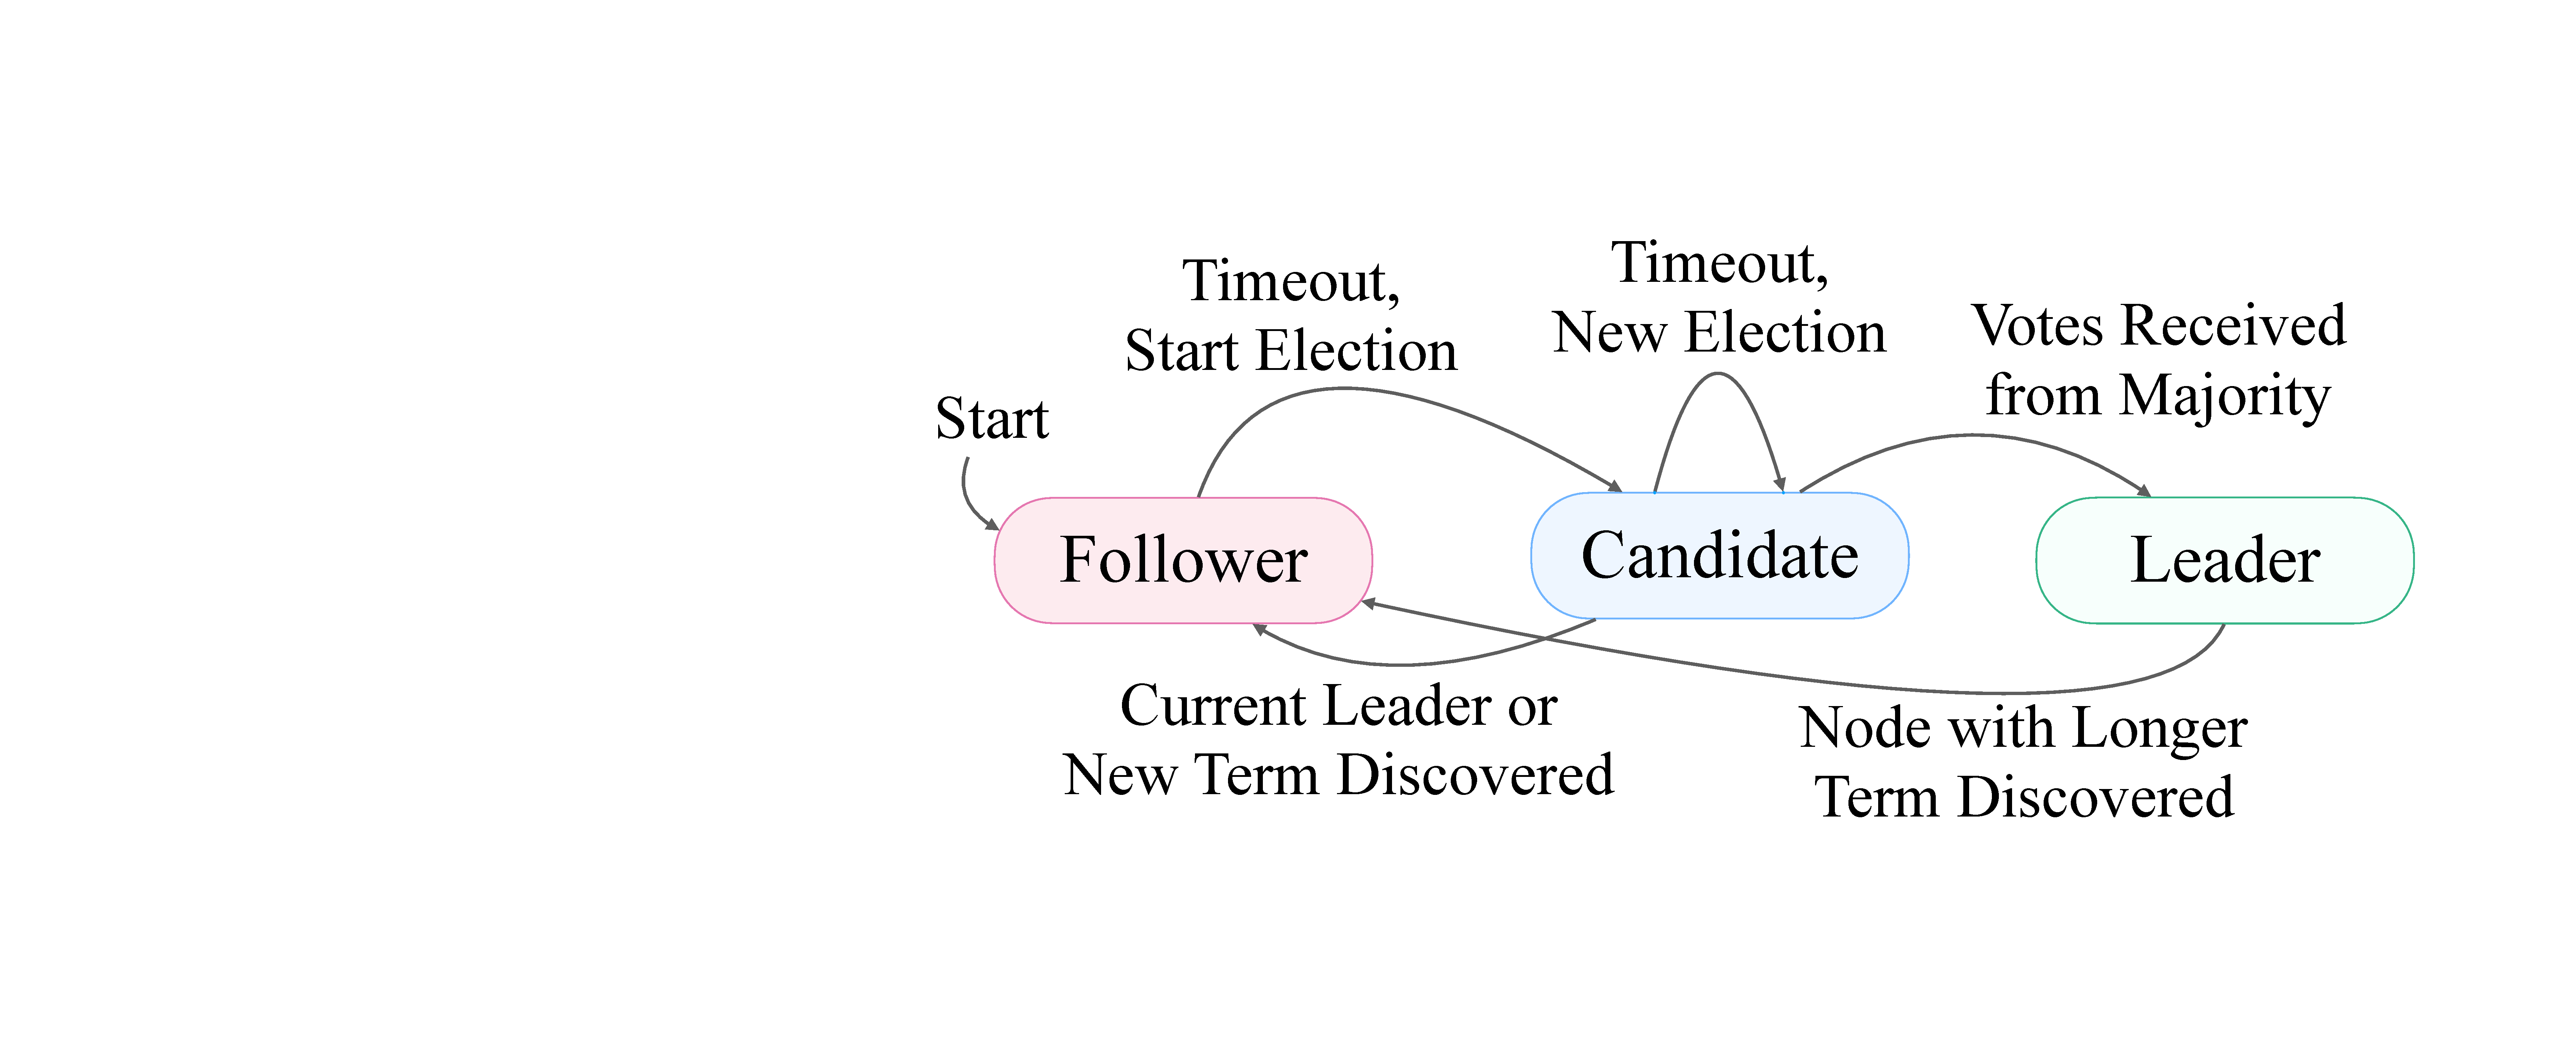
\includegraphics[width=0.6\columnwidth]{Figures/raft.pdf}
            % \vspace{- 1mm}
    \caption{Leader Election in Raft Consensus}
    \label{fig:raft}
    % \vspace{-6mm}
\end{figure}

\paragraph{Network Peers}
The network peers (nodes) have different responsibilities depending on their role and the blockchain framework. In \ac{PoW} based blockchains, these nodes are typically divided into miner nodes and validation nodes, with the former taking part in solving the \ac{PoW} hash problem on top of its validation role. In Hyperledger Fabric, the main types of peers are endorser peers (which receive the transaction proposal, run the smart contract and endorse the transaction) and the orderers that are tasked with ordering the transaction and reaching the consensus on the final block.
\paragraph{Smart Contracts (chaincodes)}
The logic of the blockchain operation is implemented as a smart contract (or chaincode in Hyperledger Fabric). This is a piece of code that either defines the terms of the transaction or an enforceable function depending on the outcome of a transaction (e.g., a penalty for not meeting a certain clause in the contract). %Smart contracts are the power behind the automatic enforcement in blockchains.
\paragraph{Channels}
Channels in Hyperledger Fabric allow the participant organizations in the network to have a virtual blockchain network within the broader blockchain network without needing to replicate the nodes (e.g., hardware resources, etc.). This enables further privacy measures for more complex transactions and logic in the blockchain. In addition, Hyperledger Fabric allows multiple ledgers per channel.
% consists of different types of entities, peer nodes, ordering service nodes and clients, belonging to various organizations. Each of these has an identity on the network which is provided by a Membership Service Provider (MSP) [9], typically associated with an organization. All entities in the network have visibility to the identities of all organizations and can verify them.






\subsection{Peer-Reviewed Dissemination}

% \subsubsection{}

 \begin{enumerate}
    
    \item \textbf{\underline{N. {Afraz}}}, F.~Slyne \emph{et~al.}, ``Evolution of Access Network Sharing and Its Role in 5G Networks,'' \emph{Applied Sciences}, vol.~9, no.~21, p. 4566, oct 2019.

    \item H.~Ahmadi, I.~Macaluso, M.~{Ruffini}, \textbf{\underline{N. {Afraz}}}, ``Blockchain Technology and Smart Contracts in 5G and Beyond Networks [Tutorial Talk],'' 2019, European Conferences on Networks and Communications (EUCNC).

    \end{enumerate}
% We first describe the manual cycle of these business processes and the challenges associated with it. Then, we model the bilateral trade of network resources in the context of smart contracts and blockchain transactions. Finally, we report and discuss the results of our experiments using Hyperledger Fabric \cite{fabric}, a permissioned blockchain framework.



% \begin{figure}
%     \centering
%     \includegraphics[width=0.49\textwidth]{figs/Fig.pdf}
%     \caption{The blockchain transaction flow}
%     \label{fig:flow}
% \end{figure}


% \subsection{Blockchain for Private Markets}
% Blockchain is a tool that provides a novel record-keeping method that is distributed, transparent, immutable, and anonymous. As a concept, blockchain challenges the blind trust on the numerous central authorities who are currently in charge of vital and critical transactions among users and enterprises. 
% Bitcoin, the most well-known use case for blockchain technology, has been known as the front face of the technology. Bitcoin is a digital asset or a cryptographic currency designed to remove the dependency on a central authority (a bank in this case) to achieve trust among its users.
% The main innovation of  Blockchain is preventing double-spending while offering a distributed alternative to the costly real-world central bank system, which provides the required mechanisms to avoid double-spending. In short, blockchain technology provides a robust solution for trustable bookkeeping.


% Blockchain technology is being considered as the primary trust solution when a trustworthy central bookkeeper is absent. Example applications are Government and Private Management, Electronic Voting, Authorship and Ownership, etc. \cite{8552978}, while more are currently under study, such as applications in pharmaceutical supply-chain \cite{7987376}, Consumer Electronics \cite{8386955}, smart-cities \cite{8386958}, privacy protection in health-care \cite{8386918} and insurance \cite{8386868}. 


% It was later realized that the cryptocurrency application does not fully utilize the potential of blockchain technology. In other words, the same decentralized consensus mechanism could be used to maintain the same level of trust for the logic-enabled transaction rather than simple bookkeeping. 

%The idea of blockchain was further complemented by the concept of smart contracts which introduced the blockchain technology, not only as a robust bookkeeping tool but also as an effective automation platform which can address many trust-related concerns in multi-party business ecosystems. A Smart Contract is an immutable piece of logic (computer program) that enhances the distributed ledger technology with self-enforcing pre-negotiated agreements.

% In this thesis, we target the blockchain's features that enables automating the inter-operator agreement and settlement processes. 

% In this section, we aim to provide a concise introduction to the different features of the blockchain and smart contracts technology. We will briefly introduce different categories of blockchains. Then we will describe different components of a blockchain application and also introduce the approaches to evaluate the performance of a blockchain application/network.

% \subsection{Blockchain Classification}






% \subsubsection{Blockchain Performance Evaluation}
% A blockchain application operates over an underlying network of different components. In \cite{10.1007/978-3-030-16946-6_5,10.1007/978-3-662-58820-8_18} the authors have proposed different distributed auction mechanisms over an Ethereum network and analyzed the performance/cost of their implementation in terms of estimated gas costs and time efficiency. 
% The main objective of a blockchain application is to handle a number of transactions that are submitted by the participants and proceed to the verification and ordering process, leading to the generation of a block and the transaction outcome being written on the ledger.
% In the context of Hyperledger blockchain frameworks the performance of the application is closely tied to the performance of each component (e.g., peers, orderers, containers, etc.) and the network that interconnects them. The performance of a blockchain application/network can be measured using the following metrics:


% \begin{itemize}
%     \item Transaction Throughput, measured in transactions per second (TPS):
%     The number of transactions that are processed by the blockchain and written on the ledger in a given second.
    
%     \begin{equation} \label{eq1}
%     \begin{split}
%     Transaction\,Throughput = \frac{Total\,Transactions}{Total\,time\,in\,seconds}
%     \end{split}
%     \end{equation}

%     \item Transaction Latency:
%     The amount of time taken from the moment when a transaction is submitted until the moment when it is confirmed and available on the blockchain. This includes the propagation time and the processing time due to the consensus/ordering mechanism.
    
%     \begin{equation} \label{eq2}
%     \begin{split}
%     Transaction\,Latency = t_{Confirmation} - t_{Submission}
%     \end{split}
%     \end{equation}


%     \item Computing Intensity:
%     The amount of computing resources consumed by the blockchain throughout the operating time, including the processing power, memory, storage, I/O and network. This metric is of great importance as it could determine the cost efficiency of a blockchain application. Furthermore, besides the capital expenditure for providing the computing capacity, blockchain networks could require huge amounts of energy to operate. Therefore, the computing intensity would also affect the operation costs of the blockchain.
    

% \end{itemize}


% The performance of three major blockchain frameworks is compared in Table. \ref{tab:bc-perform}.
% A more in-depth study of the performance metrics and evaluation methods is presented by the Hyperledger Performance and Scale Working Group  \cite{hgperf,pswg}.

% \begin{table}[htbp]
%   \caption{Performance of Blockchain Frameworks} 
%   \label{tab:bc-perform}
%   \small % text size of table content
%   \centering % center the table
%   \begin{tabular}{lcccccccr} % alignment of each column data
%   \toprule[\heavyrulewidth]\toprule[\heavyrulewidth]
%   Platform/Metric & Bitcoin    & Ethereum     &  Fabric \\ \hline
%   \midrule
%     Average Latency  & $\approx 10\, Min$ & $\approx 12.5\, Sec$ & $\approx MilliSec$      \\
%     Throughput (TPS) & 7   & 10 - 30    & 20,000 \cite{Gorenflo_2019}          \\
%   \bottomrule[\heavyrulewidth] 
%   \end{tabular}
% \end{table}




% \vspace{-1mm}

% \subsection{Blockchain Components}
% \subsection{Hyperledger Fabric Components}
